\subsection{Aprendizaje automático}

	Desde la máquina construida por Blaise Pascal en 1642 para realizar sumas, la primera computadora programable electrónica ENIAC hasta la actualidad, el hombre siempre ha demostrado interés por automatizar ciertos procesos. En particular, el tener una máquina que pudiera leer como una persona era un sueño, que tuvo sus inicios alrededor de 1914 cuando Edmund Fournier d'Albe desarrolló el \textit{Optophone} (ver figura X), que era un escaner de mano que al moverlo a través de una página impresa, producía tonos que correspondían	a letras o caracteres específicos \cite{EFdAlbe}.

			\begin{figure}[htbp]
				\centering
				\centerline{
					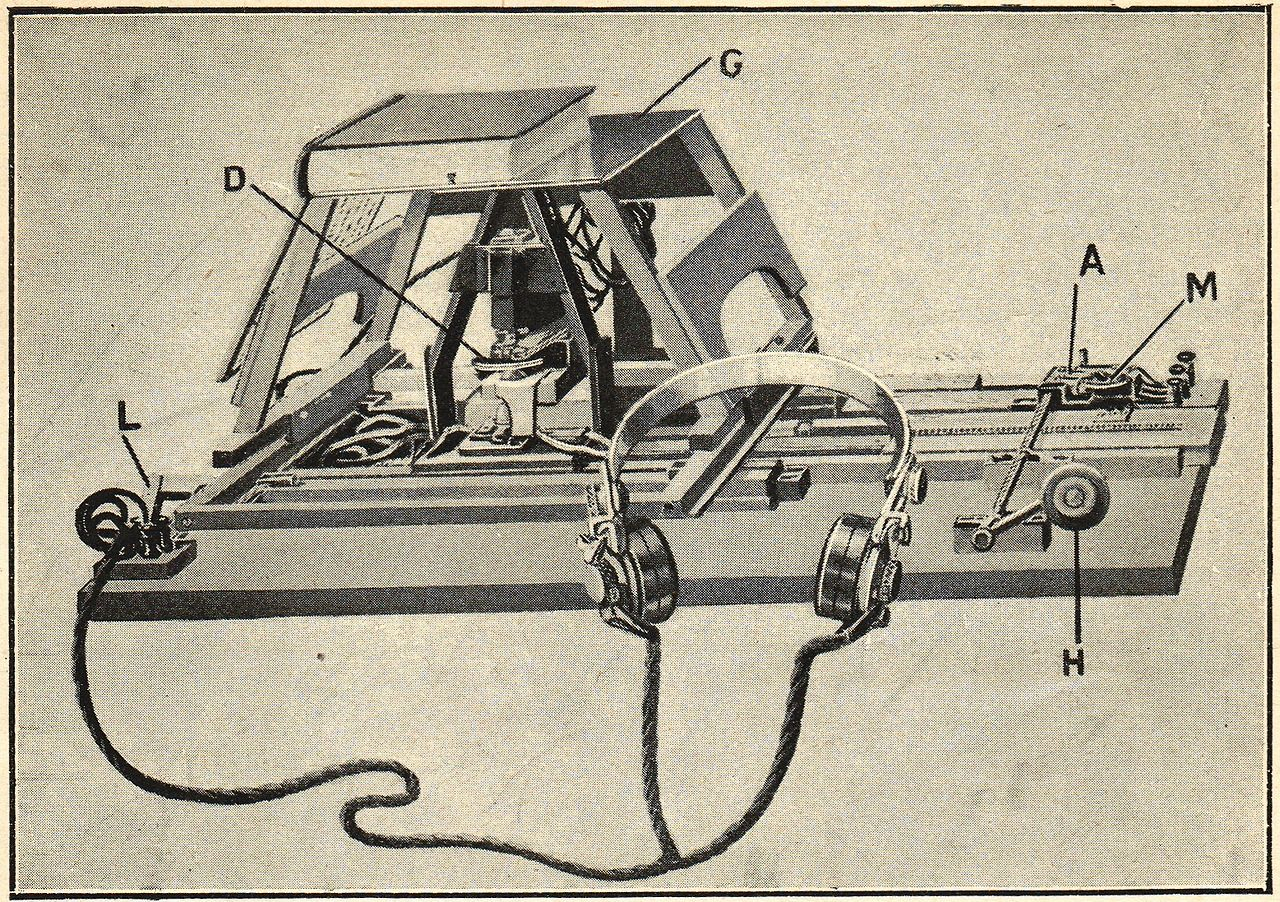
\includegraphics[scale=1]{img/Optophone.jpg}
				}
				\caption[Optophone]{Imagen del \textit{Optophone} en detalle. Extraida de la revista Vetenskapen och livet (1922).}
				\label{fig: Optophone}
			\end{figure}
			
	Durante gran parte del siglo \rom{20} y hasta el día de hoy, la cantidad de información almacenada en libros y documentos escritos ha crecido de manera exponencial. Esto se debe a que cada día se vive en un mundo más globalizado, donde la información es una herramienta fundamental en cualquier ámbito. Con el surgimiento de las primeras computadoras y la digitalización de la información, se volvió más fácil compartir datos. Sin embargo, el proceso de digitalizar los documentos ya existentes era un proceso tedioso ya que se hacía manualmente. Debido a esto, era imperativo tener algún método automático que ayudara a clasificar y analizar toda esa información ya que sobrepasaba la capacidad de las personas de hacerlo por sí mismas. Dada esta necesidad es que surge el campo de \textit{aprendizaje automático} o \textit{machine learning} para proveer métodos que resuelvan estos problemas. El aprendizaje automático estudia métodos que permiten detectar automáticamente patrones en los datos y luego usar esos patrones descubiertos para predecir datos futuros o poder tomar ciertas decisiones en condiciones de incertidumbre. 
	
	Uno de los temas que se tratan en este campo es el del reconocimiento de texto en imágenes. Las aplicaciones son muy numerosas, desde ayudar a las personas no videntes \cite{Optelec}, realizar detección de patentes \cite{DAB} o hacer traducción automática de textos en diferentes idiomas \cite{WordLens}.
	 
	 El campo de \textit{machine learning} tiene fuertes bases en la estadística por lo cual, conceptos como los desarrollados en el apéndice A sobre ``Conceptos de probabilidad y notación'' van a ser de utilidad para comprender las siguientes subsecciones.
	 
	 De todas las áreas existentes en este campo, las más destacadas e importantes son las de: aprendizaje supervisado y no supervisado. Las mismas se van a ver a continuación.
	 	
	\subsubsection{Aprendizaje supervisado}
	
	El aprendizaje supervisado es una rama del aprendizaje automático cuyo objetivo es, dado un conjunto de entradas denotado por $X$ y uno de salidas denotado por $Y$, establecer un mapeo entre $X$ e $Y$ dado un conjunto etiquetado de pares de entrada-salida $M=\{(x_i,y_i) x_i \in X, y_i \in Y \}^{N}_{i=1}$ donde $M$ es llamado el \textit{conjunto de entrenamiento} y $N$ es el número de ejemplos de entrenamiento.
	
	El conjunto de entrenamiento es un elemento indispensable en cualquier algoritmo de aprendizaje supervisado, ya que representa la base fundamental de conocimiento necesaria para que algoritmo pueda realizar futuras predicciones. En general, mientras más conocmiento se tenga sobre las características del objeto de interés que se esté analizando, más precisa va a ser la clasificación sobre nuevas entradas. Esto último hace referencia al concepto de \textit{generalización}, es decir, la habilidad de interpretar con precisión nuevas entradas luego de haber experimentado un conjunto de entrenamiento. Este conocimiento se construye a partir de la variabilidad de los objetos conocidos, es decir el poder contar con un gran conjunto de muestras que reflejen las posibles variaciones del objeto de interés. Esto le otorga robustez a la clasificación. 
	
	En la configuración más simple, cada entrada $x_i$ del conjunto de entrenamiento es un vector $D$-dimensional de números. Estas son llamadas \textit{características} (\textit{features}, de su traducción al inglés). En general, sin embargo, $x_i$ puede ser un objeto con una estructura compleja, como una imagen, un mensaje de correo, etc.
	
	Dependiendo del tipo de problema a tratar, la salida $y_i$ puede ser una variable categórica, donde $y_i \in \{1,\dots,C\}$ (conjunto finito de clases), o puede ser un valor real. Cuando $y_i$ es una variable categórica, estamos frente a un problema de \textit{clasificación} donde el objetivo es ``etiquetar'' o nombrar los objetos observados. Cuando $y_i$ es una variable real, estamos en presencia de un problema de regresión, que es similar a la clasificación excepto que la respuesta es en general una variable continua.
	
	Por ejemplo, consideremos un clasificador de caracteres alfanuméricos que tiene como conjunto de entrenamiento un grupo de imágenes que representan a cada carácter individualmente. Luego, dado que un carácter puede estar representado de diferentes formas, es decir, pueden haber variaciones en la perspectiva del mismo, en la iluminación del ambiente, el ruido de la imagen, entre otros, es necesario poder contar con la mayor cantidad de estas variaciones. Esto se debe a que mientras más conocimiento se tenga sobre las características del objeto de interés y las diferentes formas en que este puede aparecer, más certera va a ser la clasificación sobre nuevas entradas. Esto es lógico pues las nuevas entradas van a ser variaciones de los elementos que tenemos en el conjunto de entrenamiento. Es imporante que el
	

	\subsubsection{Aprendizaje no supervisado}
	
		El aprendizaje no supervisado es la otra rama del aprendizaje automático cuyo objetivo es encontrar ``estructuras interesantes'' en los datos. A diferencia del aprendizaje supervisado, no se establece qué salida se tiene que dar para cada entrada. En cambio, se busca construir modelos de la forma $p(x_i | \theta)$ donde $\theta$ es un vector de parámetros y $x_i$ es un dato de entada. La diferencia con el aprendizaje supervisado, es que hemos establecido $p(x_i | \theta)$ en vez de $p(x_i | y_i, \theta)$; es decir, el aprendizaje supervisado es una estimación condicional en la variable de interés, mientras que el aprendizaje no supervisado es una estimación no condicional.
		
		El aprendizaje no supervisado no requiere de que haya una persona que etiquete los datos manualmente, lo cual no solo es costoso, sino que además contiene relativamente poca información, sin duda no es suficiente para estimar de forma fiable los parámetros en modelos más complejos.